\chapter{Redundancy Elimination\Author{F. Chow}}
\label{chapter:pre_not_helped}
\inputpath{part3}{pre_not_helped}
\inputprogress

\section{Introduction}
\label{section:Part3:Pre_not_helped:Intro}

Redundancy elimination\index{redundancy elimination|mainidx}\index{PRE|see{redundancy elimination}} is an important category of optimizations performed by modern optimizing compilers. 
In the course of program execution, certain computations may be repeated multiple times that yield the same results. 
Such redundant computations can be eliminated by saving the results of the earlier computations and reusing instead of recomputing them later.

There are two types of redundancies: 
\emph{full} redundancy and \emph{partial} redundancy. 
A computation is fully redundant\index{redundancy elimination!full} if the computation has occurred earlier regardless of the flow of control. 
The elimination of full redundancy is also called common subexpression elimination\index{common subexpression elimination|mainidx}. 
A computation is partially redundant\index{redundancy elimination!partial} if the computation has occurred only along certain paths. 
Full redundancy can be regarded as a special case of partial redundancy where the redundant computation occurs regardless of the path taken.

There are two different views for a computation related to redundancy: 
how it is computed and the computed value. 
The former relates to the operator and the operands it operates on, which translates to how it is represented in the program representation. 
The latter refers to the value generated by the computation in the static sense
\footnote{All values referred to in this Chapter are static values viewed with respect to the program code. 
  A static value can map to different dynamic values during program execution.}. 
As a result, algorithms for finding and eliminating redundancies can be classified into being \emph{syntax-driven} or being \emph{value-driven}. 
In syntax-driven\index{redundancy elimination!syntax-driven} analyses, two computations are the same if they are the same operation applied to the same operands that are program variables or constants. 
In this case, redundancy can arise only if the variables' values have not changed between the occurrences of the computation. 
In value-based\index{redundancy elimination!value-driven} analyses, redundancy arises whenever two computations yield the same value. 
For example, $a+b$ and $a+c$ compute the same result if $b$ and $c$ can be determined to hold the same value. 
In this chapter, we deal mostly with syntax-driven redundancy elimination. 
The last section will extend our discussion to value-based redundancy elimination.

In our discussion on syntax-driven redundancy elimination, our algorithm will focus on the optimization of a lexically\index{redundancy!lexical} identical expression, like $a+b$, that appears in the program. 
During compilation, the compiler will repeat the redundancy elimination algorithm on all the other lexically identified expressions in the program.

The style of the program representation can impact the effectiveness of the algorithm applied. 
We distinguish between \emph{statements} and \emph{expressions}. 
Expressions\index{side effect!expression} computes to values without generating any side effect. 
Statements\index{side effect!statement} have side effects by potentially altering memory contents or control flow, and are not candidates for redundancy elimination. 
In dealing with lexically identified expressions, we advocate a maximal expression tree\index{expression tree} form of program representation. 
In this style, a large expression tree like $a+b*c-d$ are represented as is, without having to specify any assignments to temporaries for storing the intermediate values of the computation\footnote{The opposite of maximal expression tree form is the triplet form in which each arithmetic operation always defines a temporary.}. 
We also assume the Conventional SSA Form of program representation, in which each \phiweb\index{phiweb} (see Chapter~\ref{chapter:properties_and_flavours}) is interference-free and the live ranges of the SSA versions of each variable do not overlap. 
We further assume the HSSA (see Chapter~\ref{chapter:hssa}) form that completely models the aliasing in the program.

\section{Why partial redundancy elimination and SSA are related}
\label{section:Part3:Pre_not_helped:PRErelatedtoSSA}

Figure~\ref{fig:pre-examples} shows the two most basic forms of partial redundancy. 
In Figure~\ref{fig:pre-examples}(a), $a+b$ is redundant when the right path is taken. 
In Figure~\ref{fig:pre-examples}(b), $a+b$ is redundant whenever the back edge (see Section~\ref{sec:loop_nesting_forest}) of the loop is taken. 
Both are examples of \emph{strictly} partial redundancies\index{partial redundancy}, in which insertions are required to eliminate the redundancies. 
In contrast, a full redundancy\index{full redunddancy} can be deleted without requiring any insertion. 
\emph{Partial redundancy elimination (PRE)}\index{PRE} is powerful because it subsumes global common subexpressions and loop-invariant code motion.

\begin{figure}
\centering
%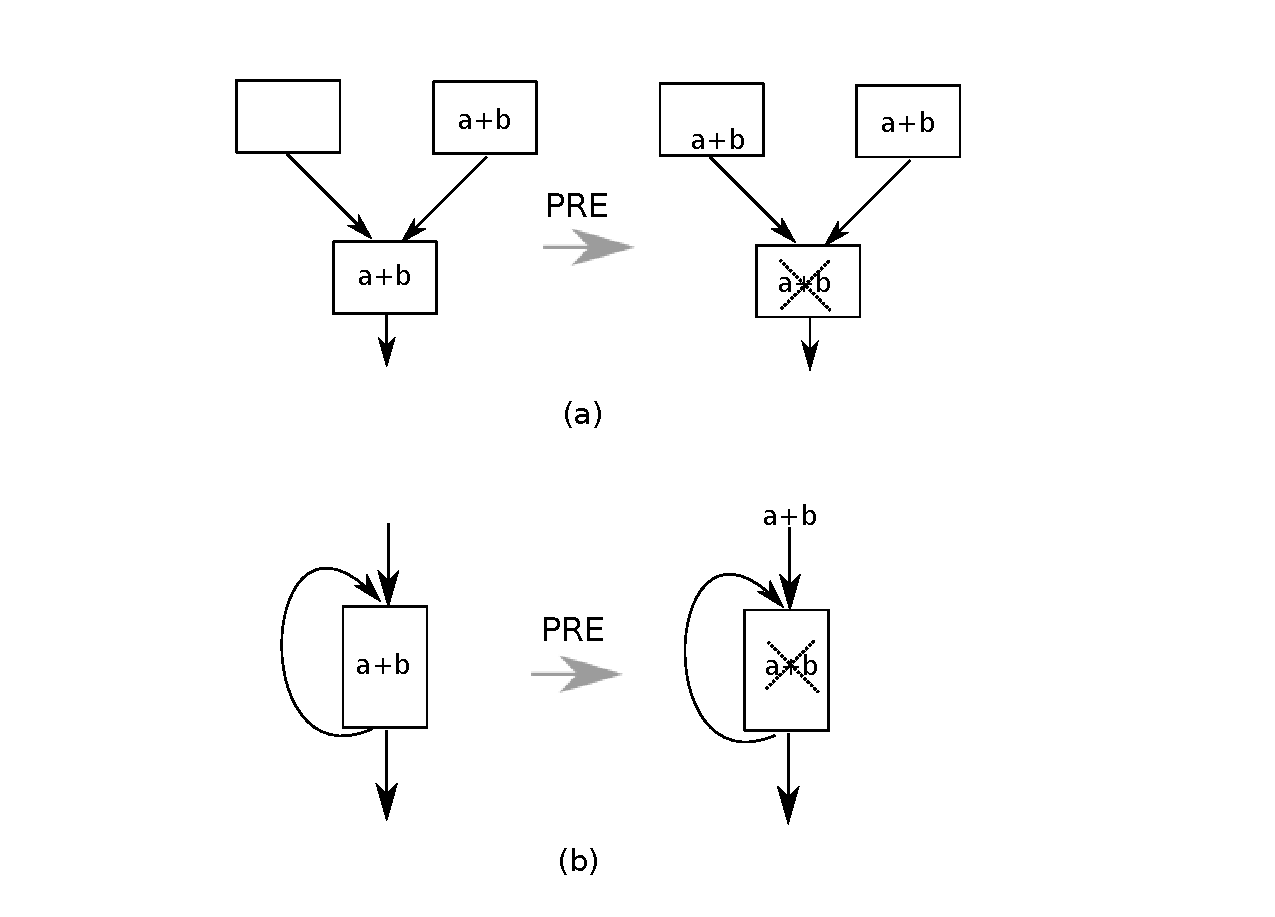
\includegraphics[scale=0.45]{fig-pre-examples.pdf}
\subfloat[First example program, before and after PRE] {
  \tikzsubfigure[1]{fig-pre-examples-ifthen}\hspace{1cm}
  \tikzsubfigure[2]{fig-pre-examples-ifthen}
}
\hfill
\subfloat[Second example program, before and after PRE] {
  \tikzsubfigure[1]{fig-pre-examples-loop}\hspace{1cm}
  \tikzsubfigure[2]{fig-pre-examples-loop}
}
\caption{Two basic examples of partial redundancy elimination.}
\label{fig:pre-examples}
\end{figure}

We can visualize the impact on redundancies of a single computation as shown in Figure~\ref{fig:ssapre-motive}. 
In the region of the control-flow graph dominated by the occurrence of $a+b$, any further occurrence of $a+b$ is fully redundant, assuming $a$ and $b$ are not modified. 
Following the program flow, once we are past the dominance frontiers, any further occurrence of $a+b$ is partially redundant. 
In constructing SSA form, dominance frontiers are where $\phi$'s are inserted. 
Since partial redundancies start at dominance frontiers, it must be related to SSA's $\phi$'s. 
In fact, the same sparse approach to modeling the use-def relationships among the occurrences of a program variable can be used to model the redundancy relationships among the different occurrences of $a+b$.

\begin{figure}
\centering
%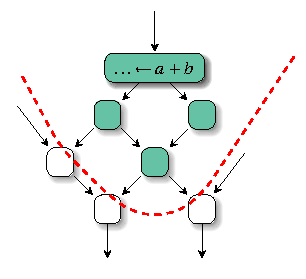
\includegraphics[scale=0.35]{fig-ssapre-motive.pdf}
\tikzfigure{fig-ssapre-motive}
\caption{Dominance frontiers (dashed) are boundaries between fully (highlighted basic blocks) and partially redundant regions (normal basic blocks).}
\label{fig:ssapre-motive}
\end{figure}

The algorithm that we present, named SSAPRE\index{SSAPRE|mainidx}, performs PRE efficiently by taking advantage of the use-def information inherent in its input conventional SSA form. 
If an occurrence $a_j+b_j$ is redundant with respect to $a_i+b_i$, SSAPRE builds a redundancy edge that connects $a_i+b_i$ to $a_j+b_j$. 
To expose potential partial redundancies, we introduce the operator $\Phi$\index{\PHIfun} at the dominance frontiers of the occurrences, which has the effect of factoring the redundancy edges at merge points in the control-flow graph.\footnote{Adhering to SSAPRE's convention, we use lower case $\phi$'s in the SSA form of variables and upper case $\Phi$'s in the SSA form for expressions.} 
The resulting \emph{factored redundancy graph}\index{factored redundancy graph} (FRG) can be regarded as the SSA form for expressions.

To make the \emph{expression SSA form}\index{expression SSA form|mainidx} more intuitive, we introduce the hypothetical temporary $h$, which can be thought of as the temporary that will be used to store the value of the expression.
The FRG can be viewed as the SSA graph for $h$.
Observe that we have not yet determined where $h$ should be defined or used. 
In referring to the FRG, a \emph{use} node will refer to a node in the FRG that is not a definition.

The SSA form for $h$ is constructed in two steps similar to ordinary SSA form: 
the $\Phi$-Insertion step followed by the Renaming step. 
In the $\Phi$-Insertion step, we insert $\Phi$'s at the dominance frontiers of all the expression occurrences, to ensure that we do not miss any possible placement positions for the purpose of PRE, as in Figure~\ref{fig:phi-insertion-a}. 
We also insert $\Phi$'s caused by expression alteration. 
Such $\Phi$'s are triggered by the occurrence of $\phi$'s for any of the operands in the expression. 
In Figure~\ref{fig:phi-insertion-b}, the $\Phi$ at block 3 is caused by the $\phi$ for $a$ in the same block, which in turns reflects the assignment to $a$ in block 2.

\begin{figure}
\centering
%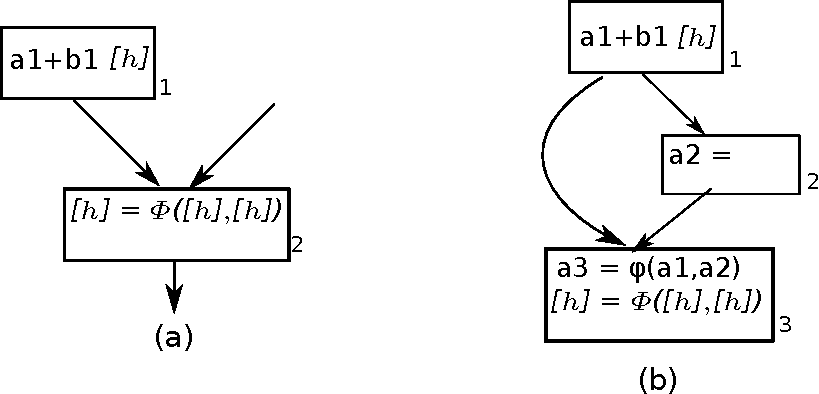
\includegraphics[scale=0.45]{fig-phi-insertion.pdf}
\subfloat[DF of expression occurrences] {
  \label{fig:phi-insertion-a}
  \tikzfigure{fig-phi-insertion-a}\hspace{1cm}
}
\subfloat[Expression alteration] {
  \label{fig:phi-insertion-b}
  \tikzfigure{fig-phi-insertion-b}
}
\caption{Examples of $\Phi$ insertion}
\label{fig:phi-insertion}
\end{figure}

The Renaming step assigns SSA versions\index{variable version} to $h$ such that occurrences renamed to identical $h$-versions will compute to the same values. 
We conduct a pre-order traversal of the dominator tree similar to the renaming step in SSA construction for variables, but with the following modifications: 
(1)~In addition to a renaming stack for each variable, we maintain a renaming stack for the expression\index{renaming, of expressions}; 
(2)~Entries on the expression stack are popped as our dominator tree traversal backtracks past the blocks where the expression originally received the version. 
Maintaining the variable and expression stacks together allows us to decide efficiently whether two occurrences of an expression should be given the same $h$-version.

There are three kinds of occurrences of the expression in the program: 
(real)~the occurrences in the original program, which we call \emph{real} occurrences; 
($\Phi$-def)~the inserted $\Phi$'s; 
and ($\Phi$-use)~the use operands of the $\Phi$'s, which are regarded as occurring at the ends of the predecessor blocks of their corresponding edges. 
During the visitation in Renaming, a $\Phi$'s is always given a new version. 
For a non-$\Phi$, i.e., cases (real) and ($\Phi$-use), we check the current version of every variable in the expression (the version on the top of each variable's renaming stack) against the version of the corresponding variable in the occurrence on the top of the expression's renaming stack. 
If all the variable versions match, we assign it the same version as the top of the expression's renaming stack. 
If any of the variable versions does not match, for case (real), we assign it a new version, as in the example of Figure~\ref{fig:rename-ifthen}; 
for case ($\Phi$-use), we assign the special class $\bot$ to the \PHIuse to denote that the value of the expression is unavailable at that point, as in the example of Figure~\ref{fig:rename-loop}. 
If a new version is assigned, we push the version on the expression stack.

\begin{figure}
\centering
%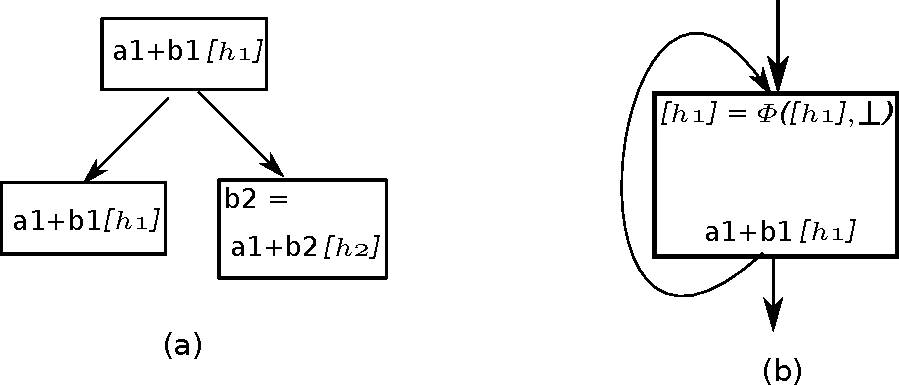
\includegraphics[scale=0.45]{fig-rename.pdf}
\subfloat[] {\tikzfigure{fig-rename-ifthen}\label{fig:rename-ifthen}}
\subfloat[] {\tikzfigure{fig-rename-loop}\label{fig:rename-loop}}
\caption{Examples of expression renaming}
\label{fig:rename}
%TODO: put [h1] & [h2] at the right place
\end{figure}
  
The FRG captures all the redundancies of $a+b$ in the program. 
In fact, it contains just the right amount of information for determining the optimal code placement. 
Because strictly partial redundancies can only occur at the \PHInodes, insertions for PRE only need to be considered at the $\Phi$'s.

\section{How SSAPRE Works}\index{SSAPRE}
\label{section:Part3:Pre_not_helped:SSAPRE}

Referring to the expression being optimized as $X$, we use the term \emph{placement} to denote the set of points in the \emph{optimized} program where $X$'s computation occurs. 
In contrast, \emph{original computation points} refer to the points in the \emph{original} program where $X$'s computation took place. 
The \emph{original} program will be transformed to the \emph{optimized} program by performing a set of \emph{insertions} and \emph{deletions}.

The objective of SSAPRE is to find a placement that satisfies the following four criteria in this order:\\
\textbf{-- Correctness}\index{PRE, correctness} $X$ is fully available at all the original computation points.\\
\textbf{-- Safety}\index{PRE, safety} There is no insertion of $X$ on any path that did not originally contain $X$.\\
\textbf{-- Computational optimality}\index{PRE, computational optimality} No other safe and correct placement can result in fewer computations of $X$ on any path from entry to exit in the program.\\
\textbf{-- Lifetime optimality}\index{PRE, lifetime optimality} Subject to the computational optimality, the life range of the temporary introduced to store $X$ is minimized.

Each occurrence of $X$ at its original computation point can be qualified
with exactly one of the following attributes:
(1)~\emph{fully redundant};
(2)~\emph{strictly partially redundant};
(3)~\emph{non-redundant}.

As a code placement problem, SSAPRE follows the same two-step process used in all PRE algorithms. 
The first step determines the best set of insertion points that render as many strictly partially redundant occurrences fully redundant as possible. 
The second step deletes fully redundant computations, taking into account the effects of the inserted computations. 
As we consider this second step to be well understood, the challenge lies in the first step for coming up with the best set of insertion points. 
The first step will tackle the safety, computational optimality and lifetime optimality criteria, while the correctness criterion is delegated to the second step. 
For the rest of this section, we only focus on the first step for finding the best insertion points, which is driven by the strictly partially redundant occurrences.

We assume that all critical edges\index{critical edge} in the control-flow graph have been removed by inserting empty basic blocks at such edges (see Algorithm~\ref{alg:ssadestruction:splitting}).
In the SSAPRE approach, insertions are only performed at \PHIuses.
When we say a $\Phi$ is a candidate for insertion, it means we will consider inserting at its use operands to render $X$ available at the entry to the basic block containing that $\Phi$. 
An insertion at a \PHIuse means inserting $X$ at the incoming edge corresponding to that $\Phi$ operand. 
In reality, the actual insertion is done at the end of the predecessor block.

\subsection{The Safety Criterion}\index{SSAPRE, safety criterion}

As we have pointed out, at the end of Section~\ref{section:Part3:Pre_not_helped:PRErelatedtoSSA}, insertions only need to be considered at the $\Phi$'s. 
The safety criterion implies that we should only insert at $\Phi$'s where $X$ is \downsafe (fully anticipated\index{fully anticipated|see{downsafe}}). 
Thus, we perform data-flow analysis on the FRG to determine the \downsafe attribute for $\Phi$'s. 
Data-flow analysis can be performed with linear complexity on SSA graphs, which we illustrate with the Downsafety computation.

A $\Phi$ is not \downsafe\index{downsafe|mainidx} if there is a control-flow path from that $\Phi$ along which the expression is not computed before program exit or before being altered by the redefinition of one of its variables. 
Except for loops with no exit, this can happen only due to one of the following cases: 
(dead) there is a path to exit or an alteration of the expression along which the $\Phi$ result version is not used; 
or (transitive) the $\Phi$ result version appears as the operand of another $\Phi$ that is not \downsafe. 
Case (dead) represents the initialization for our backward propagation of $\neg \downsafe$; 
all other $\Phi$'s are initially marked \downsafe. 
The Downsafety propagation is based on case (transitive). 
Since a real occurrence of the expression blocks the case (transitive) propagation, we define a \hasrealuse flag attached to each $\Phi$ operand and set this flag to true when the $\Phi$ operand is defined by another $\Phi$ and the path from its defining $\Phi$ to its appearance as a $\Phi$ operand crosses a real occurrence. 
The propagation of $\neg \downsafe$ is blocked whenever the \hasrealuse flag is true. 
Figure~\ref{fig:downsafety} gives the DownSafety propagation algorithm. 
The initialization of the \hasrealuse flags is performed in the earlier Renaming phase.

\begin{algorithm}
  \LinesNumbered
{
  \ForEach{$f \in$ \{$\Phi$'s in the program\}}{
    \lIf{$\exists$ path $P$ to program exit or alteration of expression along which $f$ is not used}{
      $\downsafe(f) \gets$ false\;
    }
  }
  \ForEach{$f \in$ \{$\Phi$'s in the program\}}{
    \If{{\bf not} $\downsafe(f)$}{
      \ForEach{operand $\omega$ of $f$}{
        \lIf{{\bf not} $\hasrealuse(\omega)$}{Reset\_downsafe($\omega$)}
      }
    }
  }
}
\vspace{1em}
%\Func{Reset\_downsafe($X$)}
       {
  \lIf{$\Def(X)$ is not a $\Phi$}{\Return}
  $f \gets \Def(X)$\;
  \lIf{{\bf not} $\downsafe(f)$}{\Return}
  $\downsafe(f) \leftarrow$ false\;
  \ForEach{operand $\omega$ of $f$}{
    \lIf{\textbf{not} $\hasrealuse(\omega)$}{Reset\_downsafe($\omega$)}
  }
}

\caption{DownSafety propagation}
\label{fig:downsafety}
\end{algorithm}

\subsection{The Computational Optimality Criterion}

At this point, we have eliminated the unsafe $\Phi$'s based on the safety criterion. 
Next, we want to identify all the $\Phi$'s that are possible candidates for insertion, by disqualifying $\Phi$'s that cannot be insertion candidates in any computationally optimal placement. 
An unsafe $\Phi$ can still be an insertion candidate if the expression is fully available there, though the inserted computation will itself be fully redundant. 
We define the \canbeavail\index{available, can be|mainidx} attribute for the current step, whose purpose is to identify the region where, after appropriate insertions, the computation can become fully available. 
A $\Phi$ is $\neg \canbeavail$ if and only if inserting there violates computational optimality. 
The \canbeavail attribute can be viewed as:
$$ \canbeavail(\Phi) = \downsafe(\Phi) \cup \avail(\Phi) $$

We could compute the \avail\index{available|mainidx} attribute separately using the full availability analysis, which involves propagation in the forward direction with respect to the control-flow graph. 
But this would have performed some useless computation because we do not need to know its values within the region where the $\Phi$'s are \downsafe. 
Thus, we choose to compute \canbeavail directly by initializing a $\Phi$ to be $\neg \canbeavail$ if the $\Phi$ is not \downsafe and one of its operands is $\bot$. 
In the propagation phase, we propagate $\neg \canbeavail$ forward when a $\neg \downsafe$ $\Phi$ has an operand that is defined by a $\neg \canbeavail$ $\Phi$ and that operand is not marked \hasrealuse.

After \canbeavail has been computed, it is possible to perform insertions at all the \canbeavail $\Phi$'s. 
There would be full redundancies created among the insertions themselves, but they would not affect computational optimality because the subsequent full redundancy elimination step will remove any fully redundant inserted or non-inserted computation, leaving the earliest computations as the optimal code placement.

\subsection{The Lifetime Optimality Criterion}
To fulfill lifetime optimality, we perform a second forward propagation called Later that is derived from the well-understood partial availability analysis. 
The purpose is to disqualify \canbeavail $\Phi$'s where the computation is partially available based on the original occurrences of $X$. 
A $\Phi$ is marked \later if it is not necessary to insert there because a later insertion is possible. 
In other words, there exists a computationally optimal placement under which $X$ is not available immediately after the $\Phi$. 
We optimistically regard all the \canbeavail $\Phi$'s to be \later, except the following cases: 
(real)~the $\Phi$ has an operand defined by a real computation; 
or (transitive)~the $\Phi$ has an operand that is \canbeavail $\Phi$ marked not \later. 
Case (real) represents the initialization for our forward propagation of not \later; 
all other \canbeavail $\Phi$'s are marked \later. 
The Later propagation is based on case (transitive).

\begin{figure}
\centering
%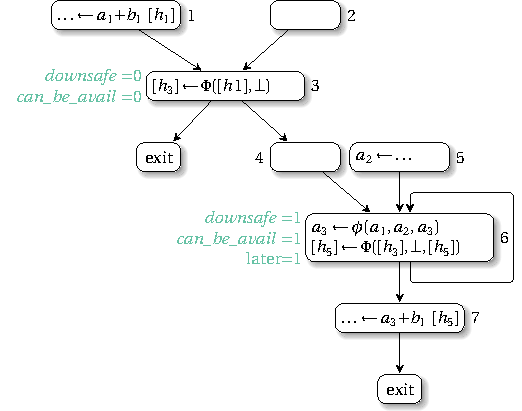
\includegraphics[scale=0.45]{fig-later-example.pdf}
\tikzfigure{fig-later-example}
\caption{Example to show the need of the \later attribute}
\label{fig:later-example}
\end{figure}

The final criterion for performing insertion is to insert at the $\Phi$'s where \canbeavail and $\neg\later$ hold. 
We call such $\Phi$'s \willbeavail. 
At these $\Phi$'s, insertion is performed at each operand that satisfies either of the following conditions:
$$
\left\lwave
\begin{array}{l}
  \textrm{it is }\bot\textrm{; or}\\
  \textrm{\hasrealuse is false and it is defined by a }\neg \willbeavail\ \Phi
\end{array}\right.
$$

We illustrate our discussion in this section with the example of Figure~\ref{fig:later-example}, where the program exhibits partial redundancy that cannot be removed by safe code motion. 
The two $\Phi$'s with their computed data-flow attributes are as shown. 
If insertions were based on \canbeavail, $a+b$ would have been inserted at the exits of blocks 4 and 5 due to the $\Phi$ in block 6, which would have resulted in unnecessary code motion that increases register pressure. 
By considering \later, no insertion is performed, which is optimal under safe PRE for this example.
 
\section{Speculative PRE}\index{PRE, speculative}
If we ignore the safety requirement of PRE discussed in Section~\ref{section:Part3:Pre_not_helped:SSAPRE}, the resulting code motion will involve speculation. 
Speculative code motion suppresses redundancy in some path at the expense of another path where the computation is added but result is unused. 
As long as the paths that are burdened with more computations are executed less frequently than the paths where the redundant computations are avoided, a net gain in program performance can be achieved. 
Thus, speculative code motion should only be performed when there are clues about the relative execution frequencies of the paths involved.

Without profile data, speculative PRE can be conservatively performed by restricting it to loop-invariant computations. 
Figure~\ref{fig:spec-pre} shows a loop-invariant computation $a+b$ that occurs in a branch inside the loop. 
This loop-invariant code motion is speculative because, depending on the branch condition inside the loop, it may be executed zero time, while moving it to the loop header causes it to execute once. 
This speculative loop-invariant code motion is profitable unless the path inside the loop containing the expression is never taken, which is usually not the case. 
When performing SSAPRE, marking $\Phi$'s located at the start of loop bodies as downsafe will effect speculative loop invariant code motion.

\begin{figure}
\centering
%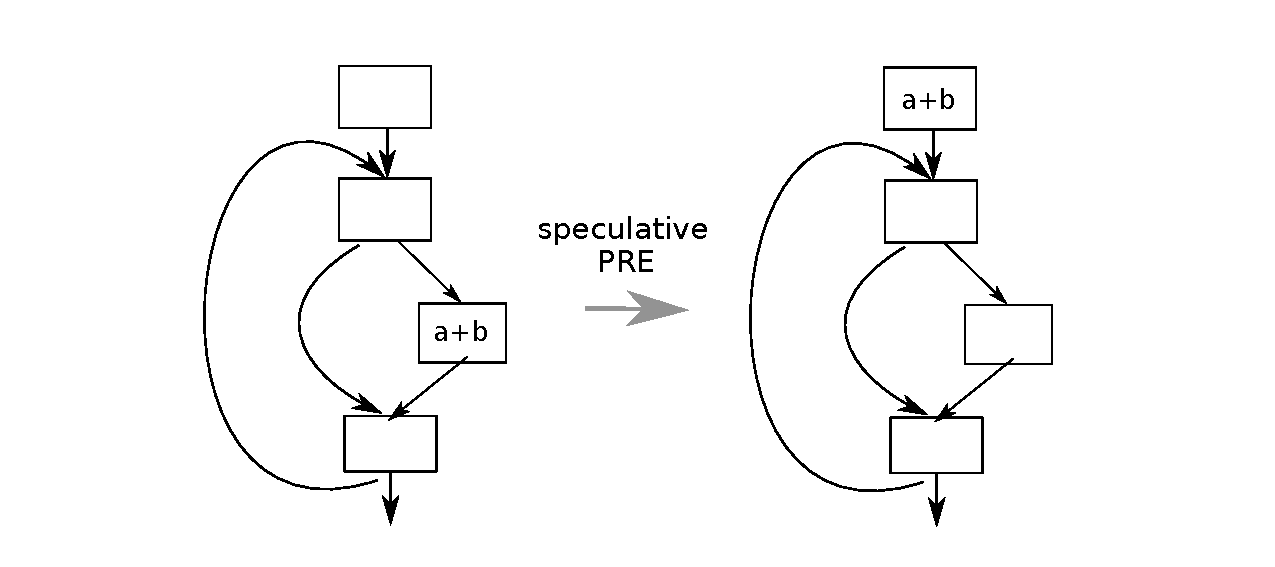
\includegraphics[scale=0.55]{fig-spec-pre.pdf}
\subfloat[Before PRE]{\tikzsubfigure[1]{fig-spec-pre}}\hspace{2cm}
\subfloat[After speculative PRE]{\tikzsubfigure[2]{fig-spec-pre}}
\caption{Speculative loop-invariant code motion}
\label{fig:spec-pre}
\end{figure}

Computations like indirect loads and divides are called \emph{dangerous} computations because they may fault. 
Dangerous computations in general should not be speculated. 
As an example, if we replace the expression $a+b$ in Figure~\ref{fig:spec-pre} by $a/b$ and the speculative code motion is performed, it may cause a runtime divide-by-zero fault after the speculation because b can be $0$ at the loop header while it is never $0$ in the branch that contains $a/b$ inside the loop body.

Dangerous computations are sometimes protected by tests (or guards) placed in the code by the programmers or automatically generated by language compilers like those for Java. 
When such a test occurs in the program, we say the dangerous computation is \emph{safety-dependent} on the control-flow point that establishes its safety. 
At the points in the program where its safety dependence is satisfied, the dangerous instruction is \emph{fault-safe}\index{fault safety} and can still be speculated.

We can represent safety dependences as value dependences in the form of abstract \tauvars. 
Each runtime test that succeeds, defines a \tauvar on its fall-through\index{fall-through} path. 
During SSAPRE, we attach these \tauvars as additional operands to the dangerous computations related to the test. 
The \tauvars are also put into SSA form, so their definitions can be found by following the use-def chains. 
The definitions of the \tauvars have abstract right-hand-side values that are not allowed to be involved in any optimization. 
Because they are abstract, they are also omitted in the generated code after the SSAPRE phase. 
A dangerous computation can be defined to have more than one \tauop, depending on its semantics. 
When all its \tauops have definitions, it means the computation is fault-safe; 
otherwise, it is unsafe to speculate. 
By including the \tauops into consideration, speculative PRE automatically honors the fault-safety of dangerous computations when it performs speculative code motion.

In Figure~\ref{fig:spec-div}, the program contains a non-zero test for $b$. 
We define an additional \tauop for the divide operation in $a/b$ in SSAPRE to provide the information whether a non-zero test for $b$ is available. 
At the start of the region guarded by the non-zero test for $b$, the compiler inserts the definition of $\tau_1$ with the abstract right-hand-side value \tauedge. 
Any appearance of $a/b$ in the region guarded by the non-zero test for $b$ will have $\tau_1$ as its \tauop. 
Having a defined \tauop allows $a/b$ to be freely speculated in the region guarded by the non-zero test, while the definition of $\tau_1$ prevents any hoisting of $a/b$ past the non-zero test.

\begin{figure}
\centering
%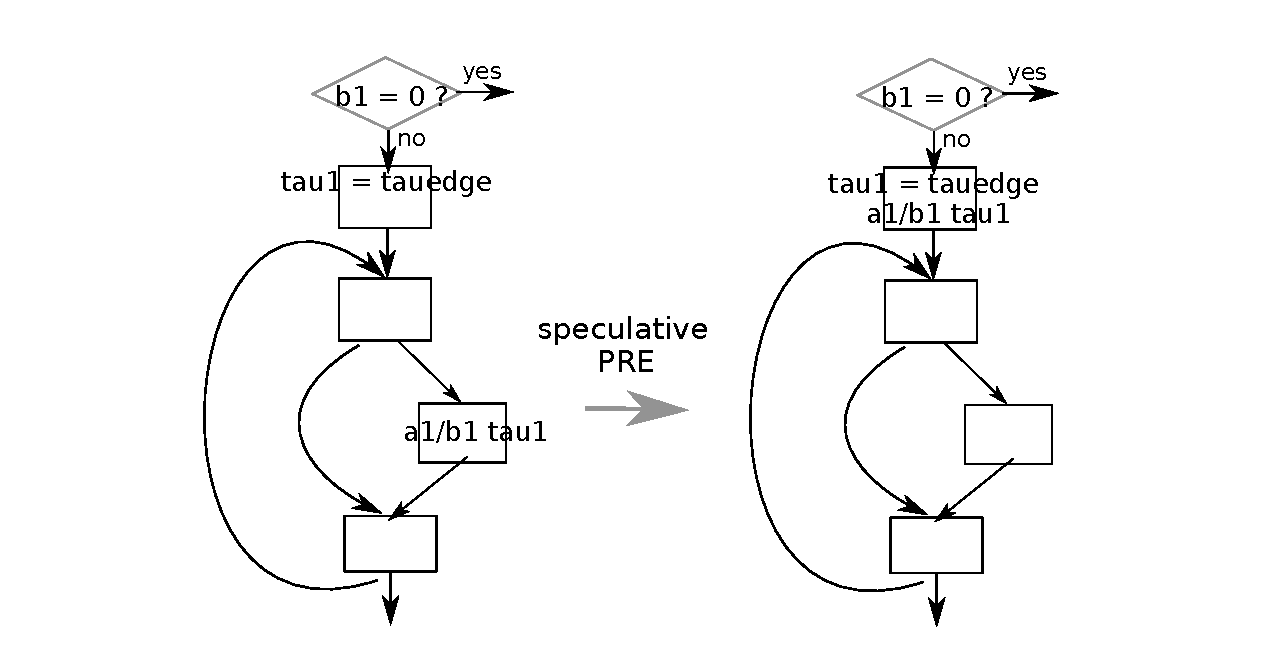
\includegraphics[scale=0.55]{fig-spec-div.pdf}
\subfloat[Before PRE]{\tikzsubfigure[1]{fig-spec-div}}\hspace{1cm}
\subfloat[After speculative PRE]{\tikzsubfigure[2]{fig-spec-div}}
\caption{Speculative and fault-safe loop-invariant code motion}
\label{fig:spec-div}
\end{figure}

\section{Register Promotion via PRE}
\index{register promotion|mainidx} Variables and most data in programs normally start out residing in memory. 
It is the compiler's job to promote those memory contents to registers as much as possible to speed up program execution.
%But when those storage contents are implicitly accessed through aliasing, it is necessary that their values are up-to-date with respect to their assigned registers.  
Load and store instructions have to be generated to transfer contents between memory locations and registers. 
The compiler also has to deal with the limited number of physical registers and find an allocation that makes the best use of them. 
Instead of solving these problems all at once, we can tackle them as two smaller problems separately:
\begin{enumerate}
\item Register promotion --- We assume there is an unlimited number of registers, called \emph{pseudo registers}\index{pseudo registers|see {pseudo registers}} (also called symbolic registers\index{symbolic registers|see{pseudo registers}}, virtual registers\index{virtual registers|see{pseudo registers}}, or temporaries\index{temporaries|see{pseudo registers}}. 
  Register promotion will allocate variables to pseudo-registers whenever possible and optimize the placement of the loads and stores that transfer their values between memory and registers.
\item Register allocation (see Chapter~\ref{chapter:register_allocation}) --- This phase will fit the unlimited number of pseudo-registers to the limited number of \emph{real} or \emph{physical} registers.
  %Because pseudo-registers have no alias, assigning them to registers involves only renaming them.  
%When it runs out of registers due to high register pressure, it will generate code to spill contents from registers back to memory.
\end{enumerate}

In this chapter, we only address the register promotion problem because it can
be cast as a redundancy elimination problem.

\subsection{Register Promotion as Placement Optimization}
Variables with no aliases are trivial register promotion candidates. 
They include the temporaries generated during PRE to hold the values of redundant computations. 
Variables in the program can also be determined via compiler analysis or by language rules to be alias-free. 
For those trivial candidates, one can rename them to unique pseudo-registers, and no load or store needs to be generated.

Our register promotion is mainly concerned with scalar variables that have aliases, indirectly accessed memory locations and constants. 
A scalar variable can have aliases whenever its address is taken, or if it is a global variable, since it can be accessed by function calls. 
A constant value is a register promotion candidate whenever some operations are using it and have to refer to it through register operands. 

Since the goal of register promotion is to obtain the most efficient placement for loads and stores, register promotion can be modeled as two separate problems: 
PRE of loads, followed by PRE of stores\index{PRE, of loads and stores}. 
In the case of constant values, our use of the term \emph{load} will extend to refer to the operation performed to put the constant value in a register. 
The PRE of stores does not apply to constants.

From the point of view of redundancy, loads behave like expressions: 
the later occurrences are the ones to be deleted. 
For stores, this is the reverse: 
as illustrated in the examples of Figure~\ref{fig:load-store-dual} the earlier stores are the ones to be deleted. 
The PRE of stores, also called \emph{partial dead code elimination}\index{dead code elimination, partial}, can thus be treated as the dual of the PRE of loads. 
Thus, performing PRE of stores has the effects of moving stores forward, while inserting them as early as possible. 
Combining the effects of the PRE of loads and stores results in optimal placements of loads and stores while minimizing the live ranges of the pseudo-registers, by virtue of the computational and lifetime optimality of our PRE algorithm.

\begin{figure}
\centering
%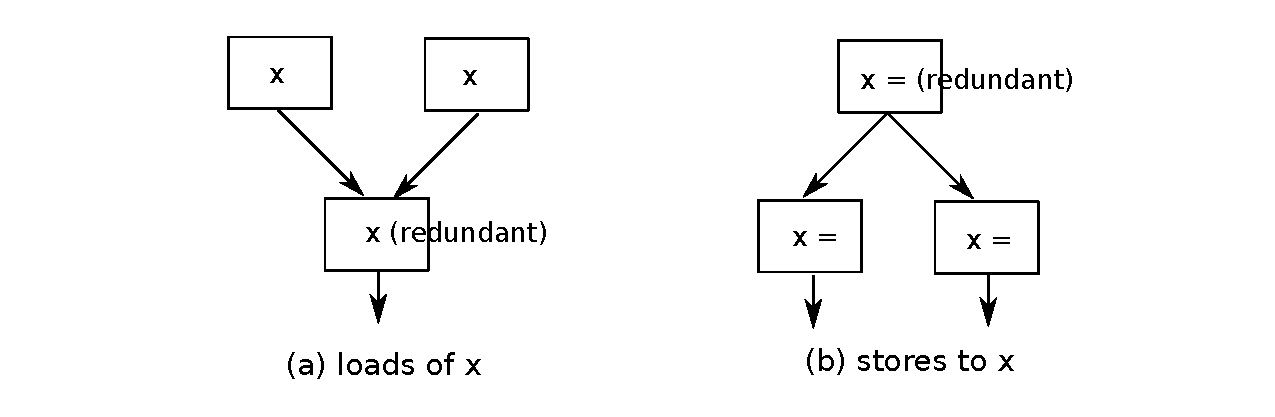
\includegraphics[scale=0.55]{fig-load-store-dual.pdf}
\subfloat[redundant load]{\tikzfigure{fig-dual-load}}\hfill
\subfloat[redundant store]{\tikzfigure{fig-dual-store}}
\caption{Duality between load and store redundancies}
\label{fig:load-store-dual}
\end{figure}

\subsection{Load Placement Optimization}
PRE applies to any computation, including loads from memory locations or creation of constants. 
In program representations, loads can either be indirect through a pointer or direct. 
Indirect loads are automatically covered by the PRE of expressions. 
Direct loads correspond to scalar variables in the program, and since our input program representation is in HSSA form, the aliasing that affects the scalar variables are completely modeled by the $\chi$ and $\mu$ functions. 
In our representation, both direct loads and constants are leaves of the expression trees. 
When we apply SSAPRE to direct loads, since the hypothetical temporary $h$ can be regarded as the candidate variable itself, the FRG corresponds somewhat to the variable's SSA graph, so the $\Phi$-insertion step and Rename step can be streamlined.

When working on the PRE of memory loads, it is important to also take into account the stores, which we call \emph{l-value} occurrences. 
A store of the form $X \leftarrow \texttt{<expr>}$ can be regarded as being made up of the sequence:
\begin{tabbing}
XX:\= while \= while \= while \= while \= while \= \kill

\> \> $r \leftarrow \texttt{<expr>}$ \\
\> \> $X \leftarrow r$ \\
\end{tabbing}
Because the pseudo-register $r$ contains the current value of $X$, any subsequent occurrences of the load of $X$ can reuse the value from $r$, and thus can be regarded as redundant. 
Figure~\ref{fig:lval-occur} gives examples of loads made redundant by stores.

\begin{figure}
\centering
%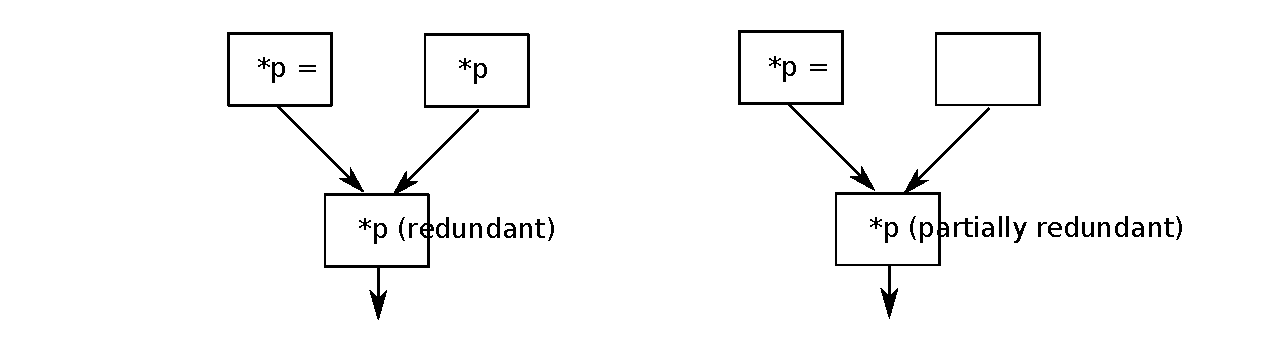
\includegraphics[scale=0.55]{fig-lval-occur}
\subfloat[]{\tikzsubfigure[1]{fig-lval-occur}}\hfill
\subfloat[]{\tikzsubfigure[2]{fig-lval-occur}}
\caption{Redundant loads after stores}
\label{fig:lval-occur}
\end{figure}

When we perform the PRE of loads, we thus include the store occurrences into consideration. 
The $\Phi$-insertion step will insert $\Phi$'s at the iterated dominance frontiers of store occurrences. 
In the Rename step, a store occurrence is always given a new $h$-version, because a store is a definition. 
Any subsequent load renamed to the same $h$-version is redundant with respect to the store.

We apply the PRE of loads (LPRE\index{PRE, of loads}) first, followed by the PRE of stores (STRE\index{PRE, of stores)}. 
This ordering is based on the fact that LPRE is not affected by the result of STRE, but LPRE creates more opportunities for the SPRE by deleting loads that would otherwise have blocked the movement of stores. 
In addition, speculation is required for the PRE of loads and stores in order for register promotion to do a decent job in loops.

The example in Figure~\ref{fig:promotion-example} illustrates what is discussed in this section. 
During LPRE, $A\gets \dots$ is regarded as a store occurrence. 
The hoisting of the load of $A$ to the loop header does not involve speculation. 
The occurrence of $A\gets\dots$ causes $r$ to be updated by splitting the store into the two statements $r\gets\dots$; $A \gets r$. 
In the PRE of stores (SPRE), speculation is needed to sink $A\gets \dots$ to outside the loop because the store occurs in a branch inside the loop. 
Without performing LPRE first, the load of $A$ inside the loop would have blocked the sinking of $A\gets \dots$.

\begin{figure}
\centering
%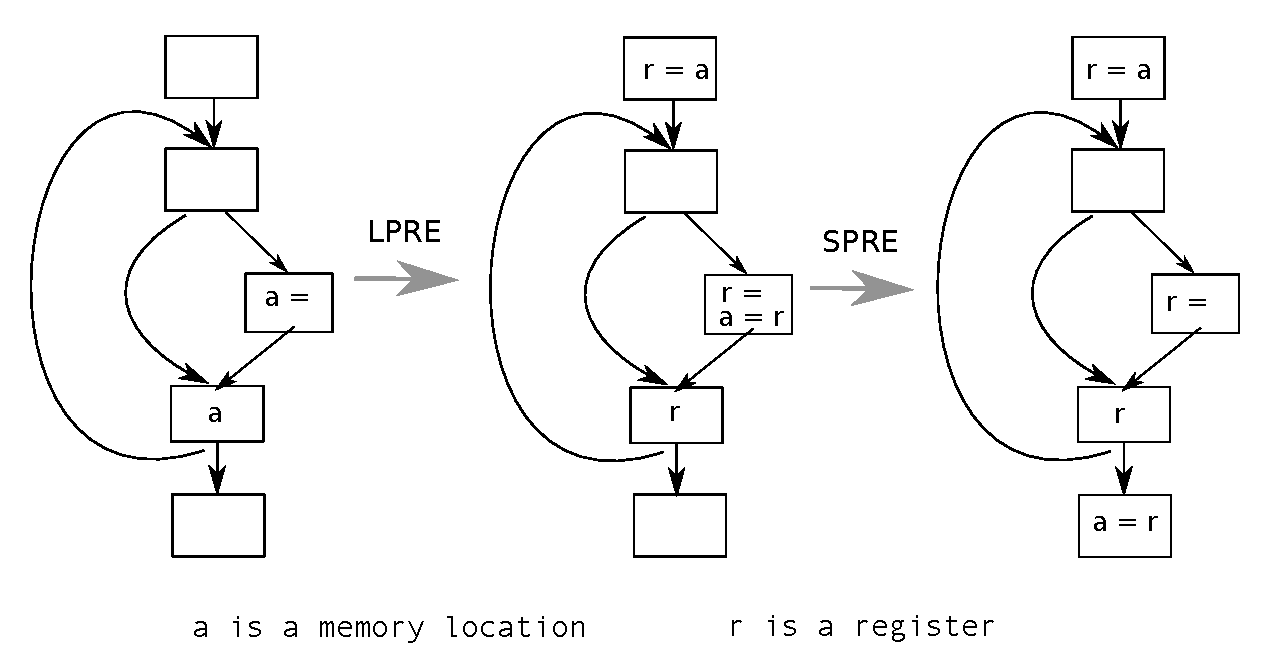
\includegraphics[scale=0.55]{fig-promotion-example.pdf}
\subfloat[original]{\tikzsubfigure[1]{fig-promotion-example}}\hfill
\subfloat[after LPRE]{\tikzsubfigure[2]{fig-promotion-example}}\hfill
\subfloat[followed by SPRE]{\tikzsubfigure[3]{fig-promotion-example}}
\caption{Register promotion via load PRE followed by store PRE}
\label{fig:promotion-example}
\end{figure}

\subsection{Store Placement Optimization}
As mentioned earlier, SPRE is the dual of LPRE. 
%In the presence of store redundancies, the earlier occurrences are redundant. 
Code motion in SPRE will have the effect of moving stores forward with respect to the control-flow graph. 
Any presence of (aliased) loads have the effect of blocking the movement of stores or rendering the earlier stores non-redundant.

To apply the dual of the SSAPRE algorithm, it is necessary to compute a program representation that is the dual of the SSA form, the \emph{static single use} (SSU)\index{SSU} form (see Chapter~\ref{chapter:ssi} -- SSU is a special case of SSI). 
In SSU, use-def edges are factored at divergence points in the control-flow graph using \sigmafuns (see Section~\ref{sub:ssi:split}).
Each use of a variable establishes a new version (we say the load \emph{uses} the version), and every store reaches exactly one load. 

We call our store PRE algorithm SSUPRE\index{SSUPRE}, which is made up of the corresponding steps in SSAPRE. 
Insertion of \sigmafuns and renaming phases, construct the SSU form for the variable whose store is being optimized. 
The data-flow analyses consist of UpSafety to compute the \emph{upsafe} (fully available) attribute, CanBeAnt to compute the \emph{can\_be\_ant} attribute and Earlier to compute the \emph{earlier} attribute. 
Though store elimination itself does not require the introduction of temporaries, lifetime optimality still needs to be considered for the temporaries introduced in the LPRE phase which hold the values to the point where the stores are placed. 
It is desirable not to sink the stores too far down.

\begin{figure}
\centering
%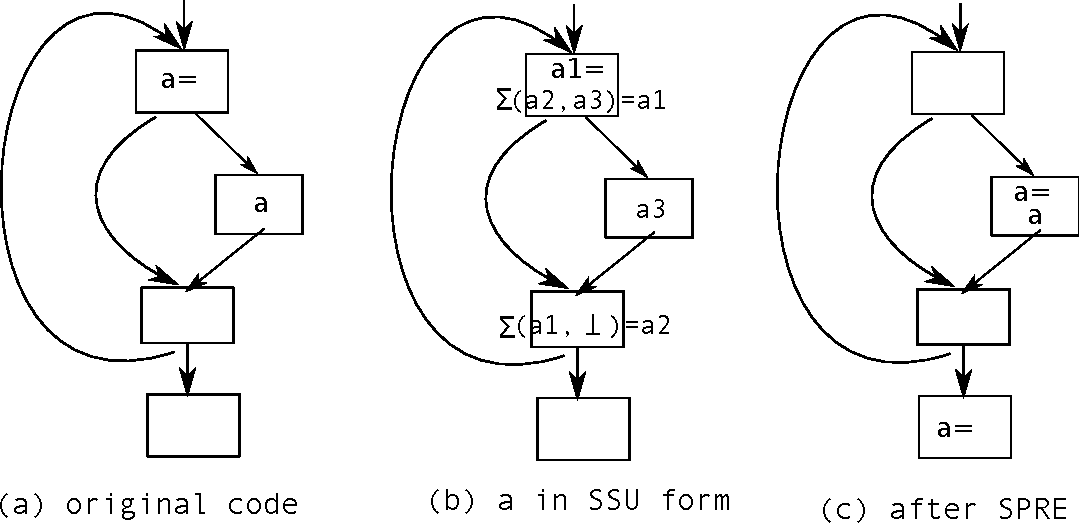
\includegraphics[scale=0.55]{fig-ssupre.pdf}
\subfloat[original]{\tikzsubfigure[1]{fig-ssupre}}\hfill
\subfloat[SSU form]{\tikzsubfigure[2]{fig-ssupre}}\hfill
\subfloat[after SPRE]{\tikzsubfigure[3]{fig-ssupre}}
\caption{Example of program in SSU form and the result of applying SSUPRE\index{static single use}}
\label{fig:ssupre}
\end{figure}

Figure~\ref{fig:ssupre} gives an example program with (b) being the SSU representation for the program in (a). 
(c) shows the result of applying SSUPRE to the code. 
The store can be sunk to outside the loop only if it is also inserted in the branch inside the loop that contains the load. 
The optimized code no longer exhibits any store redundancy.

\section{Value-based Redundancy Elimination}
\label{section:Part3:Pre_not_helped:SemanticPRE}

The redundant computations stored into a temporary introduced by PRE may be of different static values because the same lexically identified expression may yield different results at different code paths in the program. 
The PRE algorithm we have described so far is not capable of recognizing redundant computations among lexically different expressions that yield the same value. 
In this section, we discuss redundancy elimination based on value analysis.

\subsection{Value Numbering}
\label{sec:pre_not_helped:GVN}
\index{value numbering} The term \emph{value number} originated from the hash-based method developed by Cocke and Schwartz for recognizing when two expressions evaluate to the same value within a basic block. 
The value number of an expression tree can be regarded as the index of its hashed entry in the hash table. 
An expression tree is hashed recursively bottom up starting with the leaf nodes. 
Each internal node is hashed based on its operator and the value numbers of its operands. 
The local algorithm for value numbering will conduct a scan down the instructions in a basic block, assigning value numbers to the expressions. 
At an assignment, the assigned variable will be assigned the value number of the right-hand side expression. 
The assignment will also cause any value number that refers to that variable to be killed. 
For example, the program code in Figure~\ref{fig:bb-value-num}(a) will result in the value numbers $v_1$, $v_2$ and $v_3$ shown in Figure~\ref{fig:bb-value-num}(b). 
Note that variable $c$ is involved with both value numbers $v_2$ and $v_3$ because it has been redefined.

\begin{figure}[t]
\centering
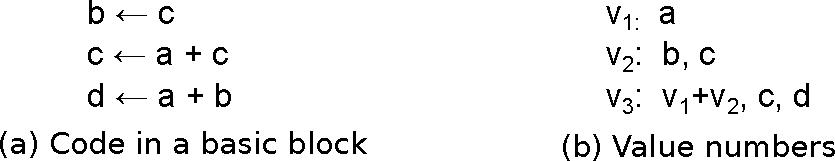
\includegraphics[scale=0.55]{fig-bb-value-num.pdf}
\caption{Value numbering in a local scope}
\label{fig:bb-value-num}
\end{figure}

\begin{figure}[t]
\centering
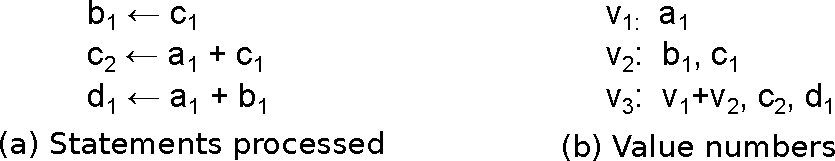
\includegraphics[scale=0.55]{fig-glob-value-num.pdf}
\caption{Global value numbering on SSA form}
\label{fig:glob-value-num}
\end{figure}

SSA form enables value numbering to be easily extended to the global scope, called global value numbering (GVN), because each SSA version of a variable corresponds to at most one static value for the variable. 
In the example of~\ref{fig:glob-value-num}, the same value numbers can be arrived at regardless of the order of processing the program code. 
One subtlety is regarding the $\phi$'s. 
When we value number a $\phi$, we would like the value numbers for its operands to have been determined. 
One strategy is to perform the global value numbering by visiting the nodes in the control-flow graph in a reverse post order traversal of the dominator tree. 
This traversal strategy can minimize the instances when a $\phi$ operand has unknown value number when the $\phi$ itself needs to be value-numbered, except in the case of back edges arising from loops. 
When this arises, we have no choice but to assign a new value number to the $\phi$. 
For example, in this loop:
\begin{tabbing}
XX:\= while \= while \= while \= while \= while \= \kill

\> \> $i_1 \leftarrow 0$; \\
\> \> $j_1 \leftarrow 0$; \\
\> \> do \{ \\
\> \> \> $i_2 \leftarrow \phi(i_3, i_1)$; \\
\> \> \> $j_2 \leftarrow \phi(j_3, j_1)$; \\
\> \> \> $i_3 \leftarrow i_2 + 4$; \\
\> \> \> $j_3 \leftarrow j_2 + 4$; \\
\> \> while \texttt{<cond>}; \\
\end{tabbing}
When we try to hash a value number for either of the two $\phi$'s, the value numbers for $i_3$ and $j_3$ are not yet determined. 
As a result, we create different value numbers for $i_2$ and $j_2$. 
This makes the above algorithm unable to recognize that $i_2$ and $j_2$ can be given the same value number, or $i_3$ and $j_3$ can be given the same value number.

The above hash-based value numbering algorithm can be regarded as pessimistic, because it will not assign the same value number to two different expressions unless it can prove they compute the same value. 
There is a different approach to performing value numbering that is not hash-based and is optimistic. 
It does not depend on any traversal over the program's flow of control, and so is not affected by the presence of back edges. 
The algorithm partitions all the expressions in the program into \emph{congruence classes}. 
Expressions in the same congruence class are considered \emph{equivalent} because they evaluate to the same static value. 
The algorithm is optimistic because when it starts, it assumes all expressions that have the same operator to be in the same congruence class. 
Given two expressions within the same congruence class, if their operands at the same operand position belong to different congruence classes, the two expressions may compute to different values, and thus should not be in the same congruence class. 
This is the subdivision criterion. 
As the algorithm iterates, the congruence classes are subdivided into smaller ones while the total number of congruence classes increases. 
The algorithm terminates when no more subdivision can occur. 
At this point, the set of congruence classes in this final partition will represent all the values in the program that we care about, and each congruence class is assigned a unique value number.

\begin{figure}[t]
\setcounter{linectr}{0}
\centering
\begin{minipage}[t]{6in}
\begin{code}
\x1 Place expressions with the same operator in the same congruence class
\x1 $N \leftarrow$ maximum number of operands among all operators in the program
\x1 $worklist \leftarrow$ set of all congruence classes
\x1 {\bf while} $worklist \neq$ \{\} 
\x2    Select and delete an arbitrary congruence class $c$ from $worklist$
\x2    {\bf for} ($p = 0; p < N; p$++)
\x3      $touched \leftarrow$ set of expressions in program that has a member of $c$ in position $p$
\x3      {\bf for} each class $s$ such that $(s \cap touched)$ is not empty and $(s \cap touched) \subset s$
\x4        Create a new class $n \leftarrow s \cap touched$
\x4        $s \leftarrow s - n$
\x4        {\bf if} $s \in worklist$
\x5           Add $n$ to $worklist$
\x4        {\bf else}
\x5           Add smaller of $n$ and $s$ to $worklist$
\end{code}
\end{minipage}
\caption{The partitioning algorithm}
\label{fig:partition-alg}
\end{figure}

The details of this partitioning algorithm is shown in Figure~\ref{fig:partition-alg}. 
At line 8, $(s \cap touched)$ being not empty implies $s$ uses a member of $c$ as its $p$th operand. 
If $(s \cap touched)$ is a proper subset of $s$, it implies some member of $s$ does not have a member of $c$ as its $p$th operand. 
This is the criterion for subdividing class $s$ because those members of $s$ that do not have a member of $c$ at its $p$th operand potentially compute to a different value. 
After the partition into $n$ and the new $s$, if $s$ is not in the worklist (i.e., processed already), the partitioning was already stable with respect to the old $s$, and we can add either $n$ or the new $s$ to the worklist to re-stabilize with respect to that split of $s$. 
Choosing the smaller one results in less overhead.

While this partition-based algorithm is not obstructed by the presence of back edges, it does have its own deficiencies. 
Because it has to consider one operand position at a time, it is not able to apply commutativity to detect more equivalences. 
Since it is not applied bottom-up with respect to the expression tree, it is not able to apply algebraic simplifications while value numbering. 
To get the best of both the hash-based and the partition-based algorithms, it is possible to apply both algorithms independently and then combine their results together to shrink the final set of value numbers.

\subsection{Redundancy Elimination under Value Numbering}
So far, we have discussed finding computations that compute to the same values, but have not addressed eliminating the redundancies among them. 
Two computations that compute to the same value exhibit redundancy only if there is an control-flow path that leads from one to the other.

An obvious approach is to consider PRE for each value number separately. 
A temporary $t$ will be introduced to store the redundant computations for each value number, but in this case, its value will stay the same throughout the lifetime of $t$. 
If there are $\phi$'s introduced for the $t$, they will be merging identical values, and we know from experience that such $\phi$'s are rare. 
A subset of such $\phi$'s is expected to come from PRE's insertions, and that implies that insertions introduced by value-number-based PRE are also rare.

Value-number-based PRE also has to deal with the additional issue of \emph{how} to generate an insertion. 
Because the same value can come from different forms of expressions at different points in the program, it is necessary to determine which form to use at each insertion point. 
If the insertion point is outside the live range of any variable version that can compute that value, then the insertion point has to be disqualified. 
Due to this complexity, and the expectation that strictly partial redundancy is rare among computations that yield the same value, it is sufficient to perform only full redundancy elimination among computations that have the same value number.

But it is possible to broaden the scope and consider PRE among lexically identical expressions and value numbers at the same time. 
In this hybrid approach, it is best to relax our restriction on the style of program representation described in Section~\ref{section:Part3:Pre_not_helped:Intro}. 
By not requiring Conventional SSA Form, we can more effectively represent the flow of values among the program variables~\footnote{We would remove the restriction that the result and operands of each $\phi$ have to be SSA versions derived from the same original program variable}. 
By regarding the live range of each SSA version to extend from its definition to program exit, we allow its value to be used whenever convenient. 
The program representation can even be in the form of triplets, in which the result of every operation is immediately stored in a temporary. 
It will just assign the value number of the right hand sides to the left-hand side variables.

This hybrid approach can be implemented based on an adaptation of the SSAPRE framework. 
Since each $\phi$ in the input can be viewed as merging different value numbers from the predecessor blocks to form a new value number, the $\Phi$-Insertion step will be driven by the presence of $\phi$'s for the program variables. 
The FRGs can be formed from some traversal of the program code. 
Each FRG can be regarded as a representation of the flow and merging of computed values based on which PRE can be performed by applying the remaining steps of the SSAPRE algorithm.

\section{Additional Reading}
The concept of partial redundancy was first introduced by Morel and Renvoise. 
In their seminal work~\cite{MR79}, Morel and Renvoise showed that global common subexpressions and loop-invariant computations are special cases of partial redundancy, and they formulated PRE as a code placement problem. 
The PRE algorithm developed by Morel and Renvoise involves bidirectional data-flow analysis, which incurs more overhead than unidirectional data-flow analysis. 
In addition, their algorithm does not yield optimal results in certain situations. 
An better placement strategy, called lazy code motion (LCM), was later developed by Knoop {\it et al}~\cite{Knoop92,Knoop94}. 
It improved on Morel and Renvoise's results by avoiding unnecessary code movements, by removing the bidirectional nature of the original PRE data-flow analysis and by proving the optimality of their algorithm. 
After lazy code motion was introduced, there have been alternative formulations of PRE algorithms that achieve the same optimal results, but differ in the formulation approach and implementation details~\cite{DS93,Dhamdhere02,Paleri03,XueKnoop06}.

The above approaches to PRE are all based on encoding program properties in bit vector forms and the iterative solution of data-flow equations. 
Since the bit vector representation uses basic blocks as its granularity, a separate algorithm is needed to detect and suppress local common subexpressions. 
Chow {\it et al}~\cite{Chow97,Kennedy99} came up with the first SSA-based approach to perform PRE. 
Their SSAPRE algorithm is an adaptation of LCM that take advantage of the use-def information inherent in SSA. 
It avoids having to encode data-flow information in bit vector form, and eliminates the need for a separate algorithm to suppress local common subexpressionsi. 
Their algorithm was first to make use of SSA to solve data-flow problems for expressions in the program, taking advantage of SSA's sparse representation so that fewer number of steps are needed to propagate data-flow information. 
The SSAPRE algorithm thus brings the many desirable characteristics of SSA-based solution techniques to PRE.

In the area of speculative PRE, Murphy {\it et al.}~\cite{Murphy08} introduced the concept of fault-safety and use it in the SSAPRE framework for the speculation of dangerous computations. 
When execution profile data are available, it is possible to tailor the use of speculation to maximize runtime performance for the execution that matches the profile. 
Xue and Cai~\cite{Xue06} presented a computationally and lifetime optimal algorithm for speculative PRE based on profile data. 
Their algorithm uses bit-vector-based data-flow analysis and applies minimum cut to flow networks formed out of the control-flow graph to find the optimal code placement. 
Zhou {et al.}~\cite{zhou11} applies the minimum cut approach to flow networks formed out of the FRG in the SSAPRE framework to achieve the same computational and lifetime optimal code motion. 
They showed their sparse approach based on SSA results in smaller flow networks, enabling the optimal code placements to be computed more efficiently.

Lo {\it et al.}~\cite{Lo98} showed that register promotion can be achieved by load placement optimization followed by store placement optimization. 
Other optimizations can potentially be implemented using the SSAPRE framework, like code hoisting, register shrink-wrap\-ping~\cite{Chow88} and live range shrinking. 
Moreover, PRE has traditionally provided the context for integrating additional optimizations into its framework. 
They include operator strength reduction~\cite{Knoop93} and linear function test replacement~\cite{Kennedy98}.

Hashed-based value numbering originated from Cocke and Schwartz~\cite{CS70}, and Rosen {\it et al.}~\cite{Rosen88} extended it to global value number based on SSA. 
The partition-based algorithm was developed by Alpern {\it et al.}~\cite{AWZ88}. 
Briggs {\it et al.}~\cite{Briggs97} presented refinements to both the hash-based and partition-based algorithms, including applying the hash-based method in a post order traversal of the dominator tree.

VanDrunen and Hosking proposed their anticipation-based SSAPRE (A-SSAPRE) that removes the requirement of Convention SSA Form and is best for program representations in the form of triplets~\cite{Vandrunen03}. 
Their algorithm determines optimization candidates and construct FRGs via a depth-first, preorder traversal over the basic blocks of the program. 
Within each FRG, non-lexically identical expressions are allowed, as long as there are potential redundancies among them. 
VanDrunen and Hosking subsequently presented their Value-based Partial Redundancy Elimination algorithm (GVN-PRE) that they claim to subsume both PRE and GVN~\cite{Vandrunen04}. 
But in this algorithm, the PRE part is not SSA-based because it uses a system of data-flow equations at the basic block level to solve for insertion points.
